\documentclass{article}
\usepackage{graphicx}
\usepackage[margin=1.5cm]{geometry}
\usepackage{amsmath}

\begin{document}
\twocolumn

\title{Wednesday Warm Up: Unit 4, AC Generators and Waveforms, Induced E-fields}
\author{Prof. Jordan C. Hanson}

\maketitle

\section{Memory Bank}

\begin{itemize}
\item $\epsilon = -N \Delta \phi_m /\Delta t$ ... Faraday's Law
\item $\phi_m = \vec{B} \cdot \vec{A} = BA \cos(\theta)$ ... Definition of magnetic flux
\item $\epsilon(t) = \epsilon_0 \sin(\omega t)$ ... AC voltage generated by generator.  $\epsilon_0$ is proportional to $\omega$.
\item $P_{max} = V_{max}^2/R$ ... Max power of an AC generator.
\item $P_{ave} = \frac{1}{2} P_{max}$ ... Average power of an AC generator.
\end{itemize}

\section{AC Generators}

\begin{enumerate}
\item Consider Fig. \ref{fig:acgen}.  Suppose that the angle between the area vector and the magnetic field is $\theta = \omega t$.  Show that
\begin{equation}
\phi(t) = BA\cos(\omega t) \label{eq:ac}
\end{equation} \vspace{1cm}
\item Given Eq. \ref{eq:ac}, it turns out that the voltage generated in the loop is proportional to $\sin(\omega t)$ and $\omega$ itself.  That is,
\begin{equation}
\epsilon(t) = BA\omega \sin(\omega t)
\end{equation}
What is the voltage at a time $t = 1/240$ seconds, $\omega = 120\pi$ Hz, $B = 0.1$ T, and $A = 0.01$ m$^2$? \\ \vspace{2cm} 
\item At what time is the voltage zero? \\ \vspace{1cm}
\item Suppose the AC generator in Fig. \ref{eq:ac} has $V_0 = 0.12$ V/Hz, so that $\epsilon(t) = V_0 \omega \sin(\omega t)$.  If the AC generator pushes current through a resistance $R = 50\Omega$, what is the \textbf{average} power generated? \\ \vspace{3cm}
\item What is the average power generated if the angular frequency is doubled?
\end{enumerate}

\begin{figure}
\centering
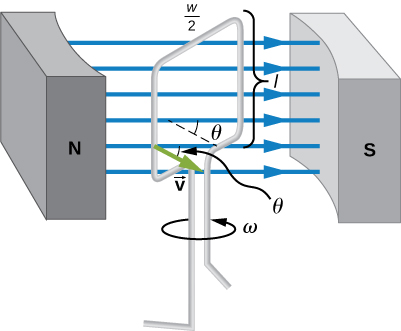
\includegraphics[width=0.3\textwidth]{figures/acGen.jpeg}
\caption{\label{fig:acgen} A schematic of the concept of an AC generator.}
\end{figure}

\section{Induced E-fields}

\begin{enumerate}
\item An eight-turn coil is tightly wrapped around the outside of the long solenoid as shown below. The radius of the solenoid is 2.0 cm and it has 10 turns per centimeter. The current through the solenoid increases according to $I = I_0\left(1-e^{-\alpha t}\right)$, where $I_0 = 4$ A, and $\alpha = 2.0\times 10^{-2}$ s$^{-1}$.  What is the emf induced in the coil when (a) $t=0$, (b) $t=100$ seconds, and (c) as $t\to \infty$? (d) Is there an induced E-field?  What is the geometry of the induced field?
\end{enumerate}

\begin{figure}
\centering
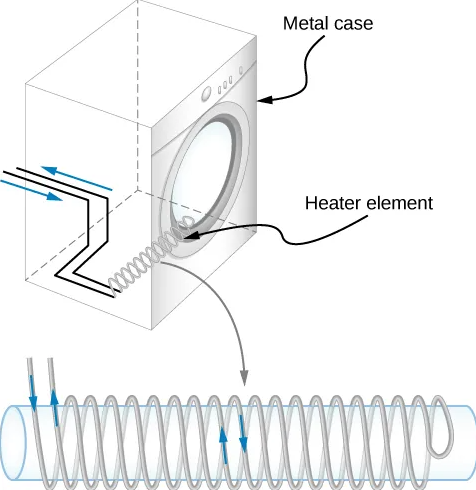
\includegraphics[width=0.3\textwidth]{figures/coils.png}
\caption{\label{fig:coils} Coils wrapped around the outside of a solenoid.}
\end{figure}

\end{document}
